% mn2esample.tex
%
% v2.1 released 22nd May 2002 (G. Hutton)
%
% The mnsample.tex file has been amended to highlight
% the proper use of LaTeX2e code with the class file
% and using natbib cross-referencing. These changes
% do not reflect the original paper by A. V. Raveendran.
%
% Previous versions of this sample document were
% compatible with the LaTeX 2.09 style file mn.sty
% v1.2 released 5th September 1994 (M. Reed)
% v1.1 released 18th July 1994
% v1.0 released 28th January 1994

\documentclass[useAMS,usenatbib]{mn2e}
\usepackage[brazilian,english]{babel}
\usepackage[utf8]{inputenc}
\usepackage[T1]{fontenc}
\usepackage{prettyref}
\usepackage{amsmath}
\usepackage{graphicx}
\usepackage{subfigure}
\usepackage{epstopdf}
\usepackage{color}
\usepackage[breaklinks=true]{hyperref}  
\usepackage{arydshln} % creates horizontal dashed lines in tables

%%%%% AUTHORS - PLACE YOUR OWN MACROS HERE %%%%%

\title[Predictions of stellar occultations by irregular satellites up to 2020]{Stellar occultation predictions for 10 irregular satellites of giant planets plus Triton up to 2020}
\author[A. R. Gomes-J\'unior, M. Assafin, L. Beauvalet et al.]{A. R. Gomes-J\'unior$^{1}$\thanks{E-mail: altair08@astro.ufrj.br},
M. Assafin$^{1,\dag}$,
L. Beauvalet$^{2,3}$,
J. Desmars$^{4}$,
R. Vieira-Martins$^{1,2,5,\dag}$,\newauthor
J. I. B. Camargo$^{2,5}$,
B. E. Morgado$^{1,2}$
F. Braga-Ribas$^{2,6}$
\\
$^{1}$Observat\'orio do Valongo/UFRJ, Ladeira Pedro Ant\^onio 43,
CEP 20.080-090 Rio de Janeiro - RJ, Brazil\\
$^{2}$Observat\'orio Nacional/MCTI, R. General Jos\'e Cristino 77, CEP 20921-400 Rio de Janeiro - RJ, Brazil\\
$^{3}$Observatoire de Paris/SYRTE, 77 Avenue Denfert Rochereau 75014 Paris, France\\
$^{4}$Institut de m\'ecanique c\'eleste et de calcul des \'eph\'em\'erides - Observatoire de Paris, UMR 8028 du CNRS, 77 Av. Denfert-Rochereau,\\ 75014 Paris, France\\
$^{5}$Laborat\'orio Interinstitucional de e-Astronomia - LIneA, Rua Gal. Jos\'e Cristino 77, Rio de Janeiro, RJ 20921-400, Brazil\\
$^{6}$Federal University of Technology - Paran\'a (UTFPR / DAFIS), Rua Sete de Setembro, 3165, CEP 80230-901, Curitiba, PR, Brazil
}
\begin{document}
\newcommand{\noccs}{5457 } % total number of occultations

\date{Accepted . Received ; in original form }

\pagerange{\pageref{firstpage}--\pageref{lastpage}} \pubyear{2016}

\maketitle

\label{firstpage}

\begin{abstract}
Due to their orbital configurations, it is common belief that the irregular satellites were probably captured by the giant planets in the early solar system. It is important to know their physical parameters, such as size, shape, albedo and composition, to trace back their true origin. The best ground-based technique to determine size and shape, and thus constrain the albedo and in a broader sense composition, is the observation of stellar occultations by these objects.
We aim to predict stellar occultations for the eight largest irregular satellites of Jupiter: Himalia, Elara, Pasiphae, Carme, Lysithea, Sinope, Ananke and Leda, and for the irregular satellites Phoebe of Saturn and Nereid of Neptune, and also for Triton.
We identified candidates to stellar occultations by the irregular satellites from the UCAC4 catalogue and from a catalogue of stars in the sky-path of Neptune obtained from observations made with the ESO2p2/WFI (2.2 m Max-Planck ESO telescope with the Wide Field Imager) instrument. These catalogues were crossed with the ephemeris of the satellites to identify stellar occultations. We used a new ephemeris based solely on the observations from \cite{GomesJunior2015} to generate predictions for the short-time future of the satellites of Jupiter. For Phoebe, we used an updated ephemeris and for Nereid and Triton we used recently published ephemeris.
We managed to identify \noccs candidates of stellar occultations between the period of January, 2016 and December, 2020. We made observational tests for the prediction of the event of Himalia in March 03, 2015. The stars and objects were observed close to the date predicted and in the same field to minimize errors and the obtained relative satellite-star positions were used to evaluate the predictions. The comparisons between the predictions and the observation tests show a good agreement. We call attention for an occultation by Triton of a bright star (R=12.5) in October 5, 2017. The event can be observed from Europe and the east coast of USA and will be a good opportunity to access the current state of the atmosphere of the satellite. We note that Jupiter will cross a populated region of stars in 2019-2020 and Saturn in 2018. This results in a large number of occultations predicted for that period.
We discuss how the successful observation of a stellar occultation by these objects is quite possible and present some of those potential occultations.
\end{abstract}

\begin{keywords}
occultations - planets and satellites: general - planets and satellites: individual: Jovian and Saturnian irregular satellites - planets and satellites: individual: Triton
\end{keywords}

\section{Introduction}\label{Sec: introducao}

Irregular satellites revolve around giant planets at large distances in eccentric, highly inclined and frequently retrograde orbits. Because of these peculiar orbits, it is largely accepted that these objects did not form by accretion around their planet, but were captured in the early solar system \citep{Sheppard2005}.

There is no consensus for a single model explaining where the irregular satellites were formed. \cite{Cuk2004} showed that the progenitor of the Himalia group may have originated in heliocentric orbits similar to the Hilda asteroid group. \cite{Sheppard2005} stated that the irregular satellites may be some of the objects that were formed within the giant planets region.

\cite{Grav2003} and \cite{Grav2007} showed that the irregular satellites from the giant planets have their colors and spectral slopes similar to C-, D- and P-type asteroids, Centaurs and trans-neptunian objects (TNOs). This suggests that they may have come from different locations in the early solar system.

\cite{Sheppard2005} and \cite{Jewitt2007} also explored the possibility that the irregular satellites originated as comets or TNOs. TNOs are highly interesting objects that, due to their large heliocentric distances, may be highly preserved with physical properties similar to those they had when they were formed \citep{Barucci2008}. This is even more true for the smaller objects, since in principle larger sizes favour physical differentiation processes in the body and vice-versa. However, due to the distance, the smaller TNOs from this region are more difficult to observe. Thus, if irregular satellites - or at least a few of them - do share a common origin with small TNOs, and since these objects are situated at much closer heliocentric distances now, this gives a unique chance of observing and studying representatives of this specific TNO population in much greater detail than could ever be possible by direct observation of this population in the Kuiper Belt. 

Phoebe is the most studied irregular satellite. \cite{Clark2005} suggest that its surface is probably covered by material of cometary origin. It was also stated by \cite{Johnson2005} that if the porosity of Phoebe is 15\%, Phoebe would have an uncompressed density similar to those of Pluto and Triton.

In order to obtain precise fundamental physical parameters like size and shape, thus constraining the albedo and in a broader sense also the composition for the irregular satellites and therefore to contribute to the study of their origin, we aim at observing stellar occultations, which provide  more accurate results than other ground-based techniques \citep{Sicardy2011, Ortiz2012, Braga-Ribas2014}. For that, reliable predictions of stellar occultations by these satellites are most needed.

We present in this paper stellar occultation predictions for the 8 major irregular satellites of Jupiter (Himalia, Elara, Pasiphae, Lysithea, Carme, Ananke, Sinope and Leda), Phoebe of Saturn and, Nereid and Triton of Neptune. Phoebe, being the most studied object with a good measured size, can be used to calibrate and evaluate the technique for similar objects.

Triton is an uncommon satellite. Its orbit is retrograde and inclined, but quasi-circular and very close to the planet compared to the irregular ones. Because Triton's orbit size is very small and its precession is not dominated by Solar perturbations, Triton is frequently excluded from the irregular satellites' class, but still studied together by many authors \citep{Sheppard2005, Jewitt2007}. Similarly to the irregular satellites, Triton was probably captured in the early solar system and may have the same origin as the TNOs \citep{Agnor2006}. However, Triton is bigger than the irregular satellites by an order of magnitude and has an atmosphere. The main motivation to study Triton by stellar occultations is to understand the evolution of its atmosphere due to Triton's complicated and extreme seasonal cycle \citep{McKinnon2007, Elliot_2000}. For all these reasons, Triton was also included as a target in this work.

Excluding Triton \citep{Olkin1997, Elliot_2000}, no observation of a stellar occultation by an irregular satellite was published up to date. Since their estimated sizes are very small (see Table \ref{Tab: satellite-diameter}), this may have discouraged earlier tries. But, in fact, given their relatively closer distances as compared to TNOs and Centaurs, and considering the current precision of their ephemeris and of star positions, we can now reliably predict the exact location and instant where the shadow of the occultation will cross the Earth. For instance, Himalia, supposedly the largest irregular satellite of Jupiter has an estimated size of 150 km \citep{Porco2003}, which is equivalent to an apparent size of about 40 mas (milliarcseconds). Thus, in this case, if the accumulated error (2 sigma or 95\% confidence level) of ephemeris and star position be around 70 mas, we have a probability of about 30\% of observing a stellar occultation, which is quite satisfactory today (see discussion in section \ref{Sec: discussion}).

\begin{table}
\caption{\label{Tab: satellite-diameter} Estimated diameter of the satellites and correspondent apparent diameter}
\begin{center}
\begin{tabular}{lccc}
\hline  \hline
\multicolumn{4}{c}{Diameter of the satellites} \tabularnewline
Satellite  & mas$^ {a}$  & km & Ref. \tabularnewline
\hline
Ananke & 8 & 29 & 1 \tabularnewline
Carme & 13 & 46 & 1 \tabularnewline
Elara & 24 & 86 & 1 \tabularnewline
Himalia & 41 & $(150\times120) \pm 20^{b}$ & 2 \tabularnewline
Leda & 5 & 20 & 1 \tabularnewline
Lysithea & 10 & 36 & 1 \tabularnewline
Pasiphae & 17 & 62 & 1 \tabularnewline
Sinope & 10 & 37 & 1 \tabularnewline
\hdashline
Phoebe & 32 & $212 \pm 1.4^{b}$ & 3 \tabularnewline
\hdashline
Nereid & 15 & $340 \pm 50^{c}$ & 4 \tabularnewline
Triton & 124 & $2707 \pm 2.0^{c}$ & 5 \tabularnewline
\hline
\end{tabular}
\end{center}
References: (1) \cite{Rettig2001}; (2) \cite{Porco2003}; (3) \cite{Thomas2010}; (4) \cite{Thomas1991}; (5) \cite{Thomas2000}.\\
$^{a}${Using a mean distance from Jupiter of 5 AU, from Saturn of 9 AU and from Neptune of 30 AU.}
$^{b}${From Cassini observations.}
$^{c}${From Voyager-2 observations.}
\par
\end{table}

\cite{GomesJunior2015} obtained 6523 suitable positions for 18 irregular satellites between 1992 and 2014 with an estimated error in the positions of about 60 to 80 mas. For some satellites the number of positions obtained is comparable to the number used in the numerical integration of orbits by the JPL \citep{Jacobson2012}. They pointed out that the ephemeris of the irregular satellites have systematic errors that may reach 200 mas for some satellites. For an object at the distance of Jupiter, this represents an error larger than 700 km in the shadow path. Using the positions obtained by \cite{GomesJunior2015} we produced a specific short-time ephemeris for the satellites of Jupiter and Phoebe to better predict stellar occultations by these objects.

Since 2009 many successful observations of stellar occultations by TNOs have been reported in the literature \citep{Elliot2010, Sicardy2011, Ortiz2012, Braga-Ribas2013}, the main disadvantages in their prediction being large heliocentric distances and ephemeris error, facts somewhat compensated for the larger diameters involved. In contrast to TNOs, the irregular satellites have much better ephemeris because the orbits of their host planets are better  known, their observational time span is much wider and covers many orbital periods. Moreover, the irregular satellites are much closer to Earth which implies in a much smaller shadow path error in kilometers. These advantages may be somewhat balanced by the smaller sizes estimated for the irregular satellites.Thus, in comparison, the chances for a successful observation of an stellar occultation by an irregular satellite should be considered at least also as good as those by TNOs.

In section \ref{Sec: integration} we show the building of the production of the new ephemeris. In section \ref{Sec: predictions}, we present the predictions of the stellar occultations by irregular satellites and how they were made. Some tests made to check the accuracy of the predictions are presented in section \ref{Sec: testes} and the final discussion is presented in section \ref{Sec: discussion}.

\section{Ephemeris} \label{Sec: integration}

In order to improve ephemeris in short time spans in the near future for a more efficient prediction of stellar occultations by irregular satellites, we need predictions based on new and recent observations. In this context, \cite{GomesJunior2015} published 6523 precise positions for 18 irregular satellites from observations made at the Observatório do Pico dos Dias (OPD), Observatoire Haute-Provence (OHP) and European Southern Observatory (ESO) between 1992 and 2014. 

Here we develop our own ephemeris based on the observations published in \cite{GomesJunior2015}. First, because the reduction was made with consistent and precise stellar catalogue and with a robust and reliable software \citep[PRAIA,][]{Assafin2011}. Second, besides recent observations, this consistent set of numerous and precise positions covers many orbital periods at many distinct orbital plane sights, so that the orbital inclinations along with all other orbital elements could be satisfactorily derived without the need of further position sets. For these reasons, only this set of positions was used for building the new ephemeris for the satellites of Jupiter.

\subsection{Special tailored Ephemerides (STE) for Jupiter irregular satellites}

The last observations used to develop JPL current ephemeris of the irregular satellites of Jupiter were obtained in 2012 \citep{Jacobson2012}. As a result, the errors in the JPL ephemeris for the current epoch are large enough to prevent accurate predictions of stellar occultations without any corrections.

Our numerical model describes the dynamical evolution of the irregular satellites of Jupiter in a jovicentric reference frame. The satellites are submitted to the influence of the Sun and the rest of the solar system, as well as that of the Galilean satellites and the first harmonics of Jupiter's gravity field. The axes of the reference frame are those of the ICRS. 

We use the following notations: \begin{itemize}
\item $i$ and $l$ one of the irregular satellites of Jupiter
\item $J$ Jupiter 
\item $j$ another body of the Solar System
\item $M_j$ the mass of the $j$-th body, not an irregular satellite
\item $m_i$ the mass of the irregular satellite $i$
\item $\vec{r_i}$ the position of the $i$-th body with respect to the barycentre of Jupiter System
\item $r_{ij}$ the distance between bodies $i$ and $j$  
\item $R_J$ the radius of Jupiter
\item $J_n$ the dynamic polar oblateness of the n-th order for Jupiter's gravity field
\item $U_{\bar{l}\hat{J}}$ potential generated by the oblateness of Jupiter on the satellite $l$
\item $\Phi_i$ is the inclination of the $i$-th satellite with respect to Jupiter's equator.
\end{itemize}

For an irregular satellite $i$, under the gravitational influence of Jupiter, the $\mathcal{N}-1$ other irregular satellites, the regular Jovian satellites and the rest of the Solar System ($\mathcal{N}$ bodies), the equation of motion is:
\begin{equation}\begin{array}{ll}

\ddot{\vec{r_i}}= & \displaystyle -GM_J\frac{\vec{r_J}-\vec{r_i}}{r_{iJ}^3}-\sum_{l=1,l\neq i}^\mathcal{N'}Gm_l\frac{\vec{r_l}-\vec{r_i}}{r_{il}^3}\\
&\displaystyle -\sum_{j=1}^\mathcal{N}GM_j \left(\frac{\vec{r_j}-\vec{r_i}}{r_{ij}^3} - \frac{\vec{r_j}-\vec{r_J}}{r_{Jj}^3} \right)\\
 & \displaystyle +GM_J \nabla U_{\bar{l}\hat{J}} -\sum_{l=1}^\mathcal{N} Gm_l\nabla U_{\bar{l}\hat{J}}
\end{array}
\label{Eq:1}
\end{equation}
where the last term in the brackets and the last term in Eq. \ref{Eq:1} represent undirect perturbations. The oblateness potential seen by the body $i$ because of Jupiter is:
\begin{equation}\begin{array}{ll}

U_{\bar{l}\hat{J}}=&\displaystyle -\frac{R_J^2 J_2}{r_{iJ}^3}\left(\frac{3}{2}\sin^2 \Phi_i-\frac{1}{2}\right)\\ &\\ & 
\displaystyle-\frac{R_J^4 J_4}{r_{iJ}^5}\left(\frac{35}{8}\sin^4 \Phi_i-\frac{15}{4}\sin^2 \Phi_i+\frac{3}{8}\right)\\
& \\
&\displaystyle-\frac{R_J^6 J_6}{r_{iJ}^7}\left(\frac{231}{16}\sin^6 \Phi_i-\frac{315}{16}\sin^4 \Phi_i+\frac{105}{16}\sin^2 \Phi_i-\frac{5}{16}\right)

\end{array}
\end{equation}

The expressions of $\nabla_lU_{\bar{l}\, \hat{i}}$ and $\nabla_i U_{\bar{i}\, \hat{l}}.$ have been developed in \citet{Lainey2004}. The equations of motion are integrated with the numerical integrator RADAU \citep{Everhart1985}. 
Our model was fitted to the observations through a least-squares procedure. The satellites were integrated one dynamical family at a time, to gain computing time, while losing minimum precision. Indeed, the interactions between satellites not belonging to the same dynamical family are negligible considering the short timespan of our integration. 

The initial osculating elements at the origin of integration are presented in Table \ref{Tab: sat_ell}.

\begin{table*}
\caption{Initial osculating elements for Jupiter irregular satellites at JD 2451545.0.
 }\label{Tab: sat_ell}
\begin{center}
\begin{tabular}{ccccccc}
\hline\hline
Satellite & a (km) & e & I$\degr$ & $\Omega\degr$ & $\omega\degr$ & $v\degr$ \\ 
\hline
Himalia &   11372100 $\pm$ 500    &    0.166 $\pm$ 0.002      &   45.14 $\pm$ 0.15      &   39.77 $\pm$ 0.19      &   351.48 $\pm$ 0.46      &   97.35 $\pm$ 0.48    \\
Elara &   11741170 $\pm$ 690  &      0.222 $\pm$ 0.002      &   28.64 $\pm$ 0.18      &   68.42 $\pm$ 0.43      &   179.82 $\pm$ 0.56      &   339.08 $\pm$ 0.82  \\
Lysithea &   11739900 $\pm$ 1300  &      0.136 $\pm$ 0.004      &    51.12 $\pm$ 0.27     &   5.53 $\pm$ 0.52      &   53.0 $\pm$ 1.5      &   318.9 $\pm$ 2.0   \\
Leda &   11140300  $\pm$ 4300  &     0.173  $\pm$ 0.007     &   16.15  $\pm$ 0.75    &   272.6  $\pm$ 1.7    &   212.2  $\pm$ 3.6          &   218.8  $\pm$ 3.2  \\
Pasiphae &  23425000  $\pm$ 5000    &     0.379  $\pm$ 0.001       &   152.44 $\pm$ 0.10      &   284.59 $\pm$ 0.21      &   135.96 $\pm$ 0.19      &   236.97 $\pm$ 0.16 \\
Sinope &   22968800 $\pm$ 5200   &     0.316 $\pm$ 0.002      &   157.76 $\pm$ 0.12      &   256.62 $\pm$ 0.55      &   298.38 $\pm$ 0.55      &   167.57 $\pm$ 0.19    \\
Carme &   24202924 $\pm$ 4800      &  0.242 $\pm$ 0.001      &   147.13 $\pm$ 0.10      &   154.01 $\pm$ 0.25      &   47.90 $\pm$ 0.29      &   234.41 $\pm$ 0.19  \\
Ananke &  21683800  $\pm$ 7200  &     0.380 $\pm$ 0.002      &   172.29 $\pm$ 0.20      &   56.9 $\pm$ 1.2      &   123.3 $\pm$ 1.2      &   231.24 $\pm$ 0.21  \\
%Themisto  & 7393800    &     0.198       &   25.77  &   220.0     &   216.3    &   262.1     \\
\hline
\end{tabular} 
\end{center}
\begin{flushleft}
\textbf{Notes}: a: semimajor axis; e : excentricity; I: inclination relative to the equatorial reference plane J2000; $\Omega$: longitude of the ascending node; $\omega$: argument of periapsis; $v$: true anomaly.
\end{flushleft}
\end{table*}

All the orbits determined for the satellites show satisfying residuals. The residuals are smaller than those obtained with JPL ephemeris, which was expected because the accuracy of an ephemeris decreases when we get further from the time of observations. The main risk of divergence over time comes from the possible absence of long-term effects when fitting to a short timespan of observations. If that were the case, our ephemeris would diverge too quickly to be of any use. JPL ephemerides are fitted over all the available observations. As a result, they will diverge less quickly than our own. Though they are no longer precise enough for our use, they remain a precious reference to identify whether our own model presents a quick divergence.

We compared our ephemeris to the JPL for all the Jupiter satellites we fitted, until 2018. For instance, the divergence between 2015 and 2018 is at most 98 mas in $\Delta \alpha \cos \delta$ and 58 mas in $\Delta \delta$ for Himalia and 181 mas in $\Delta \alpha \cos \delta$ and 152 mas in $\Delta \delta$ for Carme.

Fig. \ref{Fig: JPL-STE} displays the offsets of the positions published by \cite{GomesJunior2015} for the satellite Carme in declination relative to our ephemeris, to \cite{Jacobson2012} JUP300 JPL ephemeris and \cite{Emelyanov2008} ephemeris.We see that the systematic JPL ephemeris offsets pointed out by \cite{GomesJunior2015} are reduced with our ephemeris, as expected.

\begin{figure}
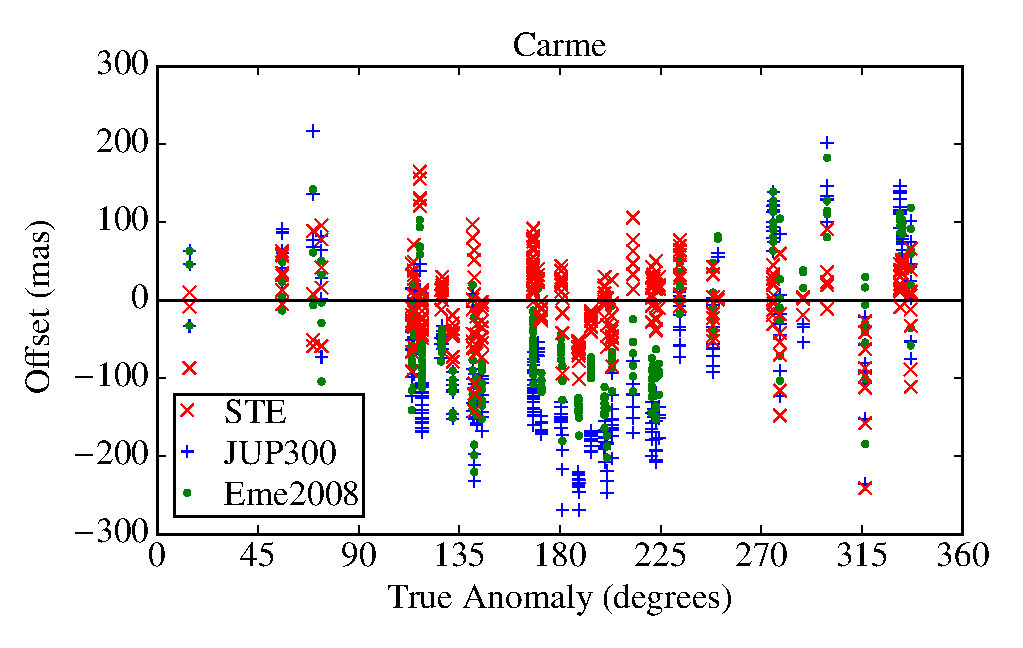
\includegraphics[width=8.8cm]{figures/Carme_ephemeris.eps}
\caption{Offsets in declination of the positions published by \protect\cite{GomesJunior2015} for Carme. The red "x" relative to the special-tailored ephemeris, the blue "+" relative to the JUP300 JPL ephemeris and the green dot relative to \protect\cite{Emelyanov2008}. As expected, the ephemeris systematic errors pointed out by \protect\cite{GomesJunior2015} are reduced with the STE ephemeris. \label{Fig: JPL-STE}}
\end{figure}

The obtained ephemeris is hereafter refered as STE, for special-tailored ephemeris.

\subsection{Phoebe's ephemeris}

For the specific case of Phoebe, the ninth satellite of Saturn, we have updated the ephemeris published in \cite{Desmars2013}. The new ephemeris (PH15) used the same dynamical model, including the perturbations of the Sun and the eight planets, the eight major satellites of Saturn and the $J_2$ parameter. The observations used to fit the model are identical to \cite{Desmars2013} (including 223 Cassini observations) with additional observations from \cite{GomesJunior2015}, \cite{Peng2015}, observations from Minor Planet Circulars between 2012 and 2014 (available on the Natural Satellite Data Center\footnote{\url{http://lnfm1.sai.msu.ru/neb/nss/bsapoouf.htm}}), and observations from Flagstaff \citep{NOFS} between 2012 and 2014. It represents a total number of 5886 observations from 1898 to 2014.

In Fig. \ref{Fig:eph-Phoebe} we compare our ephemeris (PH15) with the SAT375 JPL\footnote{Jacobson, R.A. 2015-Feb-27. "Satellite Ephemeris: SAT375", JPL Satellite Ephemeris File Release, \url{ftp://ssd.jpl.nasa.gov/pub/eph/satellites/nio/LINUX_PC/sat375l.txt}} ephemeris. The difference between them is smaller than 30 mas (< 10 mas in Declination). This difference is smaller than the apparent diameter of Phoebe (see Table \ref{Tab: satellite-diameter})

\begin{figure}
\begin{centering}
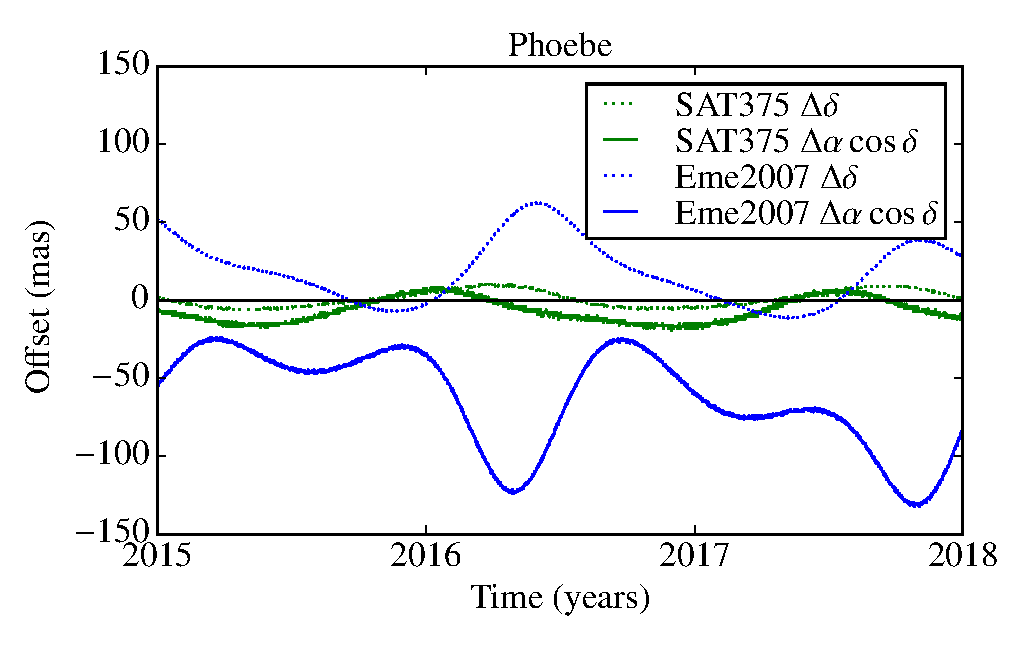
\includegraphics[width=8.8cm]{figures/Phoebe.eps} 
\caption{Comparison between the PH15, SAT375 JPL and \protect\cite{Emelyanov2007} ephemeris for the satellite Phoebe.}
\label{Fig:eph-Phoebe}
\end{centering}
\end{figure}

\subsection{Triton's and Nereid's ephemeris}

For Triton, we used the most recent ephemeris published by \cite{Emelyanov2015}. In Fig. \ref{Fig:eph-Triton} we compare it with the ephemeris published in \cite{Zhang2014} and the NEP081 JPL ephemeris \citep{Jacobson2009}. The offsets between the three ephemeris are smaller than 15 mas for the period 2015-2018. This value is much smaller than the apparent size of Triton (124 mas, see Table \ref{Tab: satellite-diameter}), which indicates a good probability of observing an event by this object.

\begin{figure*}
\begin{centering}
\subfigure[NEP081 JPL and \protect\cite{Emelyanov2015}]{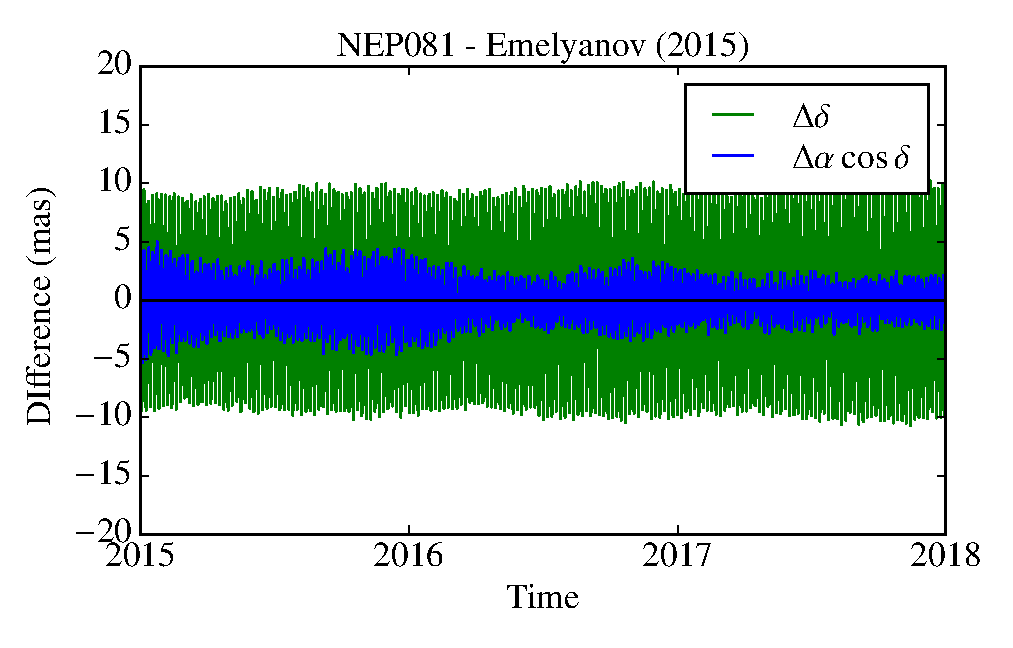
\includegraphics[width=8.7cm]{figures/JPL-EME_Triton.eps} \label{Fig:eph-Triton-eme}}
\subfigure[\protect\cite{Zhang2014} and \protect\cite{Emelyanov2015}]{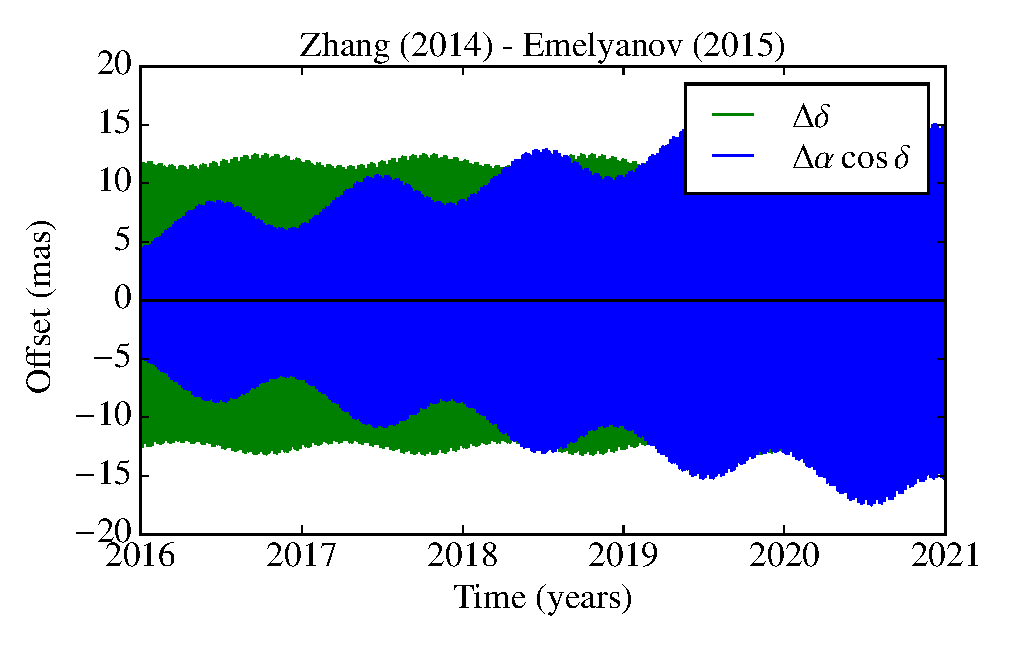
\includegraphics[width=8.7cm]{figures/Zhang-EME_Triton.eps} \label{Fig:eph-Triton-zhang}}
\caption{Comparison between the \protect\cite{Emelyanov2015}, \protect\cite{Zhang2014} and NEP081 JPL \protect\citep{Jacobson2009} ephemeris for the satellite Triton.}
\label{Fig:eph-Triton}
\end{centering}
\end{figure*}

For Nereid, we used the ephemeris published by \cite{Emelyanov2011}, which uses more recent observations than the JPL ephemeris published by \cite{Jacobson2009}. The comparison between the two ephemeris can be seen in Fig. \ref{Fig:eph-Nereid}. The right ascension offsets between them are smaller than 60 mas and the declination ones are smaller than 15 mas. For Nereid, ephemeris errors in right ascension translate to uncertainties in the central instant of a stellar occultation, so offsets of 60 mas are not critical. The declination ephemeris offsets are of the order of the apparent diameter (15 mas, see Table \ref{Tab: satellite-diameter}), resulting in fair chances (50\%) that the shadow crosses the expected Earth latitude predicted for an occultation. 

\begin{figure}
\begin{centering}
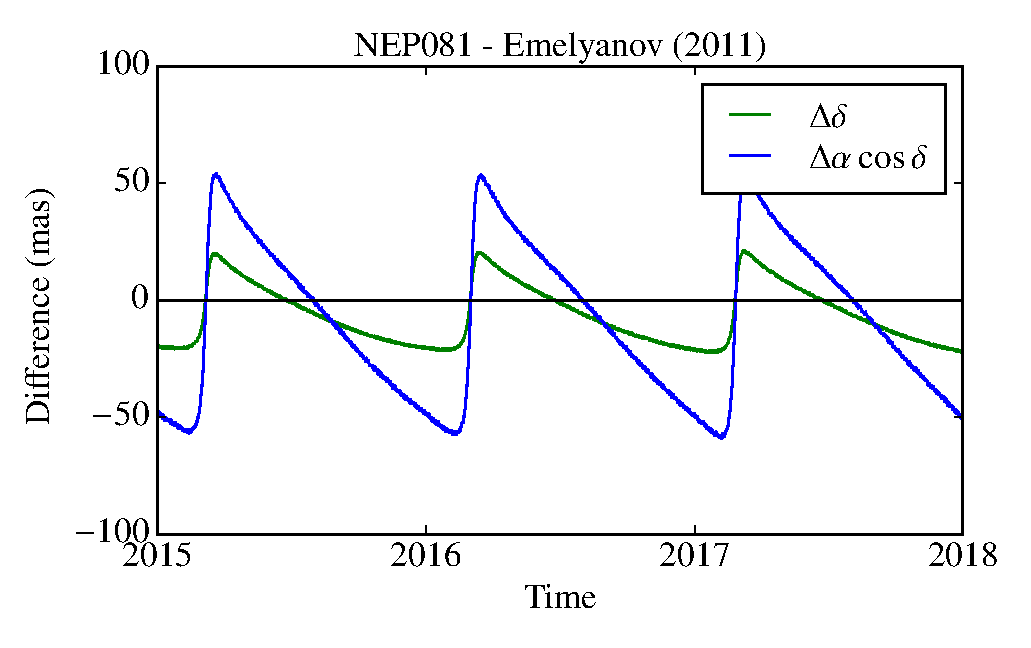
\includegraphics[width=8.8cm]{figures/JPL-EME_Nereid.eps}
\caption{Comparison between the \protect\cite{Emelyanov2011} and NEP081 JPL \protect\citep{Jacobson2009} ephemeris for the satellite Nereid.}
\label{Fig:eph-Nereid}
\end{centering}
\end{figure}

\cite{GomesJunior2015} published 902 new positions for Nereid from observations between 1992 and 2014. The development of a better ephemeris for Nereid using these new positions in the context discussed here of near future stellar occultations is desirable, but is out of the scope of this paper.  

\section{Prediction of occultations} \label{Sec: predictions}

The prediction of the occultations was made by crossing the stellar coordinates and proper motions of the UCAC4 catalogue \citep{Zacharias2013} with the ephemeris presented in Sec. \ref{Sec: integration}. The search for stellar candidates follows the same procedure as presented by \cite{Assafin2010, Assafin2012} and \cite{Camargo2014}.

We predicted occultations for the 8 major irregular satellites of Jupiter,  Ananke, Carme, Elara, Himalia, Leda, Lysithea, Pasiphae and Sinope, and for Phoebe of Saturn and Triton and Nereid of Neptune.

For Triton and Nereid, the candidates for stellar occultations in 2016 were searched using the WFI catalogue in the same way as the predictions for Centaurs and TNOs occultations by \cite{Assafin2010, Assafin2012} and \cite{Camargo2014}. This catalogue contains the stars in the path of Neptune in the sky up to mid-2016. The catalogue was generated by observations made at the ESO 2p2 telescope (IAU code 809) using the Wide Field Imager (WFI) CCD mosaic detector. The filter used was the broad-band R filter ESO\#844 with $\lambda_c$ = 651.725 nm and $\Delta\lambda$ = 162.184 nm.

A total of \noccs events were identified between January 2016 and December 2020. In Table \ref{Tab: satellite-occultation} we present the number of stellar occultations predicted by year for each satellite. Table \ref{Tab: occ-list} shows a sample of the catalogue of occultations generated and their parameters, which are necessary to produce occultation maps. Since these objects are very small, the duration of each event is a few seconds. All the occultation tables and maps will be publicly available at the CDS. No star brighter than MagR*=18 will be occulted by Triton in 2016. For this satellite, we cut events with stars fainter than R=18, since for Triton the flux drop during such an occultation would be very small. In Fig. \ref{Fig: ocultacao} we show an example of an occultation map. This is one of the only two found occultation by Triton and it will happen in October 05, 2017. This event can be observed from Europe and the east coast of USA and will be a great opportunity to study in high resolution the atmosphere of the satellite.

\begin{table}
\caption{\label{Tab: satellite-occultation} Number of stellar occultations for each satellite from January, 2016 up to December, 2020.}
\begin{centering}
\begin{tabular}{lcccccc}
\hline  \hline
%\multicolumn{4}{c}{Diameter of the satellites} \tabularnewline
Satellite  & 2016 & 2017 & 2018 & 2019 & 2020 & Total \tabularnewline
\hline
Ananke & 12 & 16 & 49 & 359 & 187 & 623 \tabularnewline
Carme & 20 & 14 & 30 & 369 & 220 & 653 \tabularnewline
Elara & 14 & 16 & 33 & 305 & 193 & 561 \tabularnewline
Himalia & 15 & 12 & 54 & 257 & 230 & 568 \tabularnewline
Leda & 8 & 24 & 38 & 362 & 208 & 640 \tabularnewline
Lysithea & 16 & 11 & 35 & 330 & 212 & 604 \tabularnewline
Pasiphae & 20 & 19 & 44 & 362 & 206 & 651 \tabularnewline
Sinope & 15 & 21 & 34 & 356 & 256 & 682 \tabularnewline
\hdashline
Phoebe & 32 & 98 & 238 & 79 & 13 & 460 \tabularnewline
\hdashline
Nereid & 11$^{a}$ & 1 & 1 & 0 & 0 & 13 \tabularnewline
Triton & -- & 1 & 1 & 0 & 0 & 2 \tabularnewline
\hline
\end{tabular}
\par \end{centering}
$^{a}$ {Using the WFI catalogue as explained in Sec. \ref{Sec: predictions}}.
\end{table}

\begin{table*}
\caption{\label{Tab: sample-cds} A sample of stellar occultation predictions for Pasiphae}
\begin{center}
\begin{tabular}{cccrcccrcrr}
\hline
\hline
d m Year~~~~h~~m~~~s & RA~~~(ICRS)~~~Dec & C/A & P/A & $\nu$ & {\it D} & $R^*$ & $\lambda$ & LST & $\mu_{\alpha*}$ & $\mu_{\delta}$ \tabularnewline
\hline
% & \multicolumn{2}{c}{Mean errors} & Nr & Nr &  UCAC4       \tabularnewline
09 04 2016 03:58:19. & 11 14 36.7707 +07 39 20.7610 & 1.003 &  17.9 & -12.88 &  4.54 & 14.9 & 271. & 22:03 &  12. & -33. \tabularnewline 
13 06 2016 00:16:12. & 11 12 48.5020 +07 06 43.3520 & 0.661 &  30.0 & +14.32 &  5.50 & 13.9 & 262. & 17:45 &  -1. &   1. \tabularnewline 
27 06 2016 13:56:09. & 11 18 03.4160 +06 23 45.1940 & 1.707 &  28.0 & +20.29 &  5.74 & 11.7 &  44. & 16:53 &   4. & -10. \tabularnewline 
18 07 2016 15:07:24. & 11 28 15.5076 +05 05 31.8060 & 0.942 &  26.7 & +27.80 &  6.05 & 14.0 &   8. & 15:40 &   4. &   4. \tabularnewline 
22 07 2016 16:15:07. & 11 30 30.4310 +04 48 43.4340 & 0.644 & 206.5 & +29.04 &  6.11 & 14.6 & 348. & 15:27 &  23. & -24. \tabularnewline 
24 07 2016 01:37:34. & 11 31 17.8471 +04 42 49.0540 & 0.029 & 206.6 & +29.46 &  6.12 & 15.1 & 206. & 15:22 &   2. &  -8. \tabularnewline 
24 07 2016 17:37:18. & 11 31 40.7472 +04 39 57.5060 & 0.840 &  26.5 & +29.66 &  6.13 & 14.9 & 326. & 15:20 & -11. &  -1. \tabularnewline 
\hline
\end{tabular}
\end{center}
\begin{flushleft}
\textbf{Notes}. Entries included: day of the year and UTC time of the prediction; right ascension and declination of the occulted star - at the central instant of occultation (corrected by proper motions); C/A: the geocentric closest approach, in arcseconds; P/A: the satellite position angle with respect to the occulted star at C/A, in degrees (zero at north of the star, increasing clockwise); $\nu$: velocity in the plane of sky, in km s$^{-1}$: positive = prograde, negative = retrograde; {\it D}: planet range to Earth, in AU; $R^*$: normalized magnitude to a common shadow velocity of 20 km s$^{-1}$ by the relationship $\textrm{R}^* = \textrm{R}_{\textrm{actual}} + 2.5 \times \log 10 \left(\frac{\textrm{velocity}} {20 \textrm{km}\, \textrm{s}^{-1}} \right)$; $\lambda$: east longitude of subplanet point in degrees, positive towards east; LST: UT + $\lambda$: local solar time at subplanet point, hh:mm; $\mu_{\alpha *}$ and $\mu_{\delta}$: proper motions in right ascension and declination, respectively (mas/year).
\label{Tab: occ-list}
\end{flushleft}
\end{table*}

\begin{figure}
\begin{centering}
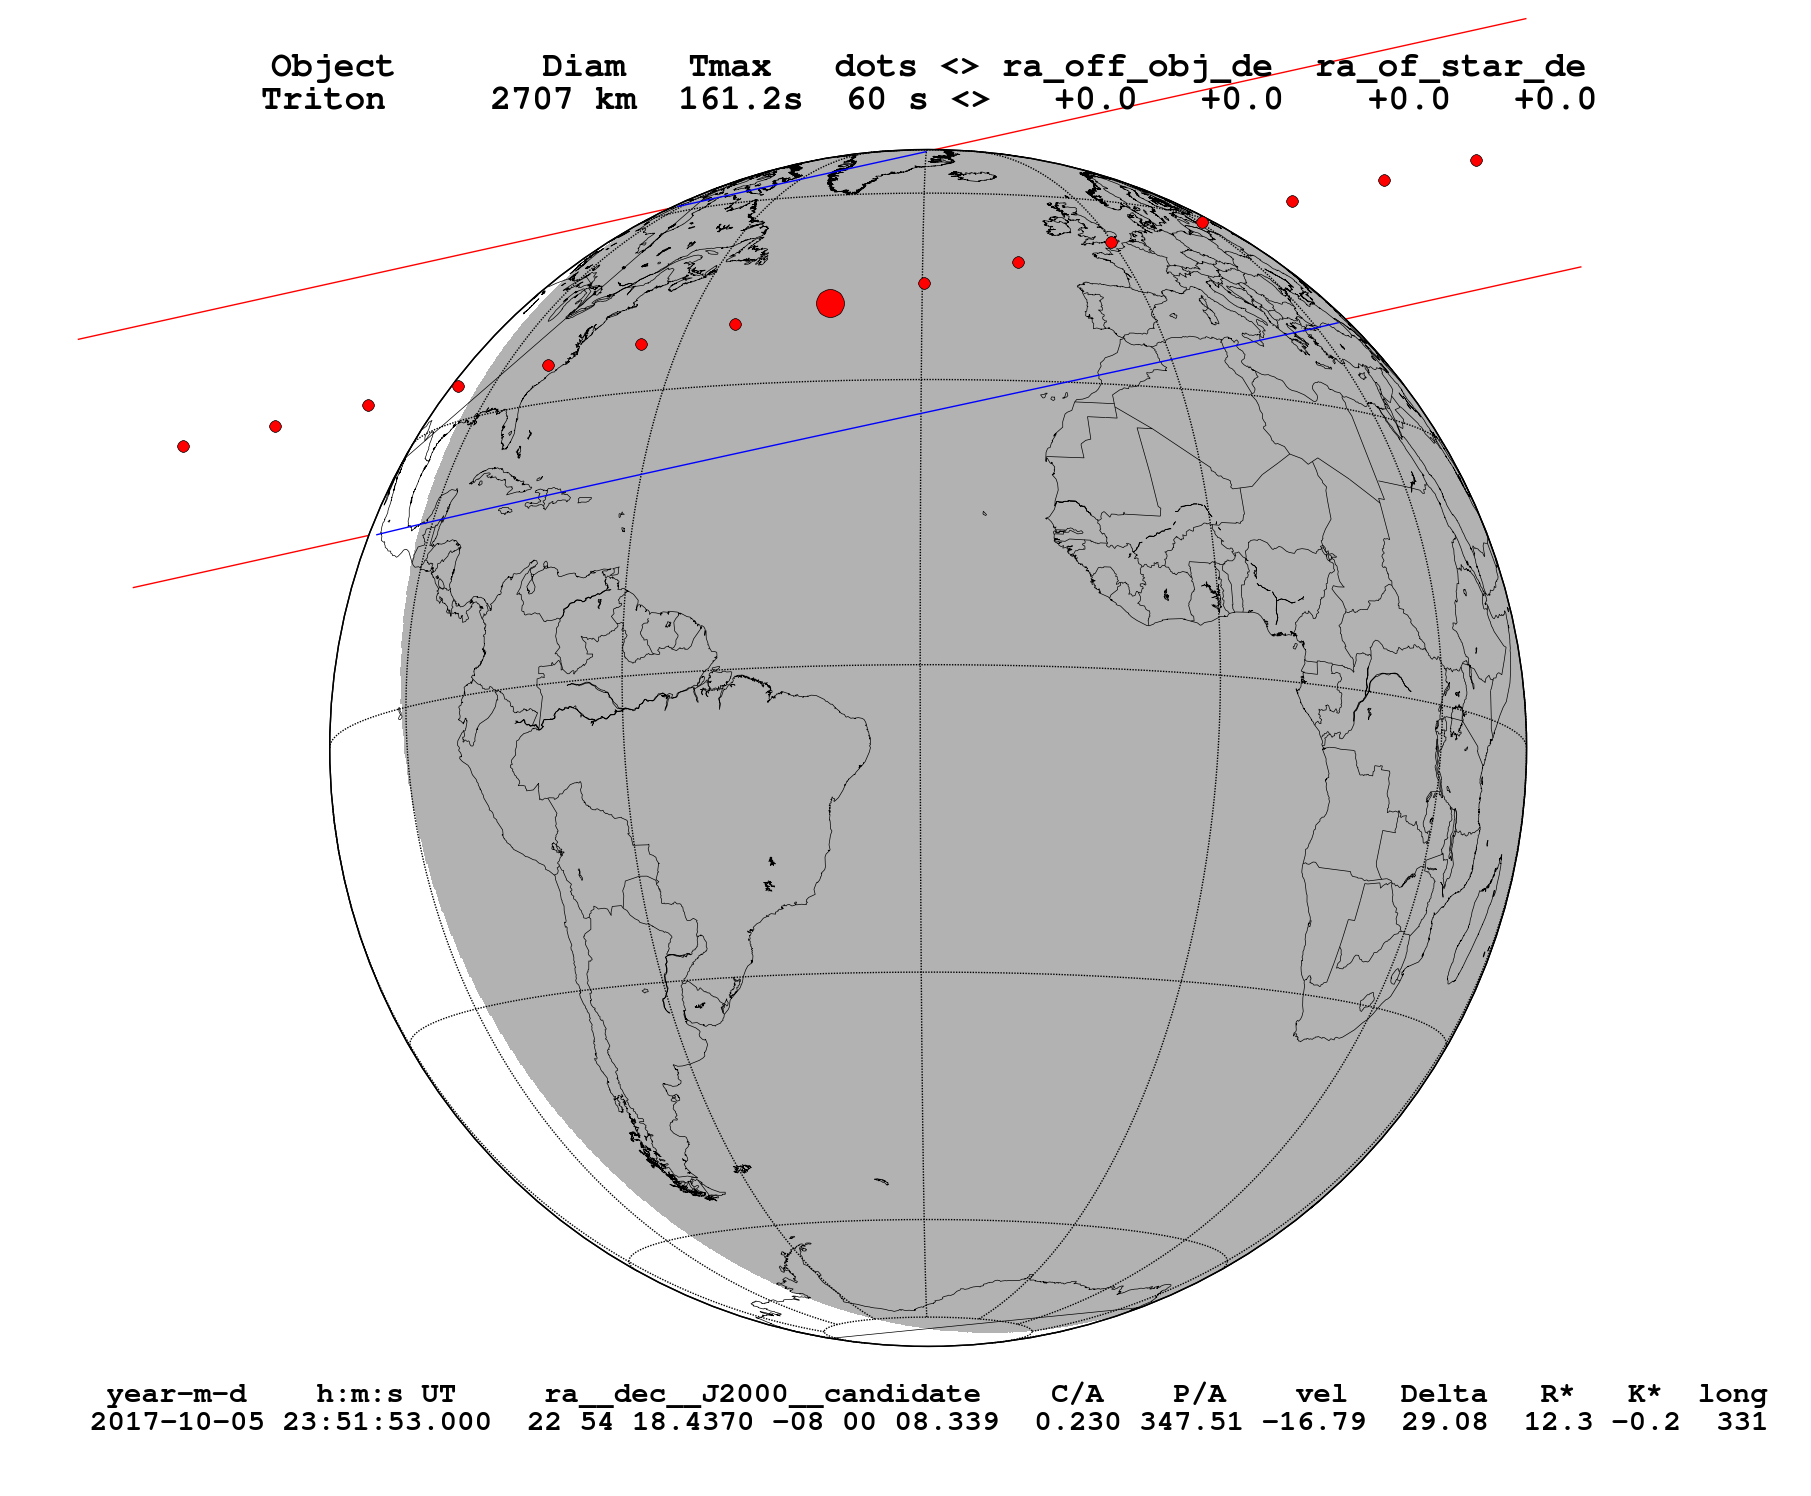
\includegraphics[width = 8.8cm]{figures/Triton_2017-10-05T23:51:53.png}   
\caption{Occultation map for Triton.% regarding to the first event sampled in Table \ref{Tab: occ-list}.
The central red dot show the geocentric closest approach of the shadow. The small ones shows the center of the shadow separated by 60s. The lines show the path of the shadow over the Earth. The shadow moves from right to left.
\textbf{Labels:} Diam: Diameter of the object; Tmax: Maximum duration of the event for a central observation; C/A: the geocentric closest approach, in arcseconds; P/A: the satellite position angle with respect to the occulted star at C/A, in degrees; vel: velocity of event in km/s; Delta: Geocentric distance to the occulting object in AU; $R^*$: normalized magnitude to a common shadow velocity of 20 km s$^{-1}$; long: east longitude of subplanet point in degrees, positive towards east.}
\label{Fig: ocultacao}
\end{centering}
\end{figure}

The first preliminary catalogue version of the ESA astrometry satellite GAIA \citep{deBruijne2012} is expected to be released up to the end of 2016 (The catalogue with five-parameter astrometric solutions is up to the end of 2017). The precise star positions to be derived by GAIA will provide better predictions with the main source of error being the ephemeris. Astrometric reduction of observations published in \cite{GomesJunior2015} will be revised with the GAIA catalogue and the predictions will be improved. Since we cannot foresee exactly when the GAIA catalogue will be released and when new and re-reduced satellite positions in the GAIA frame will become available, we decided to publish predictions up to the end of 2020. In the GAIA era, the occultation predictions will be updated.


\subsection{Prediction test} \label{Sec: testes}

Observing a stellar occultation demands a great effort. And, in our case, the shadow covers a very restricted area on Earth because of the size of the irregular satellites. Since no stellar occultation by an irregular satellite was observed up to date, with the exception of Triton, and since we want to be sure that we can start observational campaigns with reasonable chances of success, we tested an occultation prediction for a large target, to assess the quality of the prediction.

The test design consisted in observing the object and star to be occulted near the date of the event predicted when the two objects were present in the same field of view (FOV), close to each other. Thus, the relative positions between the two objects had minimal influence of the errors of the reference catalogue of stars used and possible field distortions \citep[and references therein]{Peng2008}. The relative positions of the star and satellite were used to check the original predictions. Notice that in the test we do not attempt to observe any actual occultation. The test could be performed at any site, regardless of the Earth location where the occultation would in fact be visible. 

We tested the occultation by Himalia predicted to occur on March 3, 2015. The shadow would cross the northern part of South America. For the event, four situations were considered:
\begin{enumerate}[I]
\item Our nominal, published prediction with the STE ephemeris (see Sec. \ref{Sec: integration}), and the nominal UCAC4 position of the star;
\item Prediction with the JPL ephemeris and the nominal UCAC4 position of the star;
\item From star and satellite offsets calculated from observations made a few days before the occultation when the objects were very separated (different FOVs);
\item Same as 3 but with the star and the satellite close in the same FOV.
\end{enumerate}

Table \ref{Tab: comparison-Himalia} shows the differences between the predictions in the four situations. For situation 3 we observed the objects on February 22 with the Zeiss telescope (diameter = 0.6m; FOV = $12\farcm6$; pixel scale = $0\farcs37 / pixel$) at the Observatório do Pico dos Dias, Brazil (OPD, IAU code 874, 45\degr 34\arcmin 57\arcsec W, 22\degr 32\arcmin 04\arcsec S, 1864m). On that day, Himalia and the star were observed in separate FOVs as they were still far apart. On the night of the event, March 3, the objects were observed with Perkin-Elmer telescope (diameter = 1.6m; FOV = $5\farcm8$; pixel scale = $0\farcs17 / pixel$) at OPD just over an hour after the time scheduled for the event. Satellite and star were separated by about 16 arcsec, so very close to each other (situation 4). From the calculated offsets, the center of the shadow was obtained. Notice that the shadow path was not predicted to cross the OPD (which was located at almost 2000 km south from the shadow path). This was not necessary for testing the prediction.

The critical parameter in the comparisons is the C/A, which here is related to latitudes. The apparent radius of Himalia is about 20 mas (see Table 1). In the context of the test, for a 0 mas offset in C/A we would have 100\% probability of observing the occultation, and 0\% in the case of a C/A offset equal to or larger than 20 mas, the radius of Himalia. From Table 5, we have nearly 0\% probability of success in situation 3, for which the offset in C/A was -20 mas, but when the relative astrometry was poor, 10 days prior to the event. Once at the day of the event in situation 4, the C/A offset dropped to -9 mas only, corresponding to a 55\% probability of success. Comparison with the prediction using the JPL ephemeris (situation 2) gives a +11 mas C/A offset, or a compatibility of 45\% between the ephemerides. All this suggests that there was a good probability of observing the event. The largest differences between the shadows of the four situations were 36s in time along the shadow path and 101km (31 mas) in the direction perpendicular to the shadows, suggesting that observers should be spread in narrow latitude ranges 100 km wide.

\begin{table}
\caption{\label{Tab: comparison-Himalia} Comparison between the predictions of the Himalia occultation at March 03, 2015.}
\begin{centering}
\begin{tabular}{lccc}
\hline  \hline
\multicolumn{4}{c}{Differences with respect to the STE prediction} \tabularnewline
Method  & Instant of C/A  & C/A & Sit.   \tabularnewline
\hline
STE & 00:39:51 UTC & $0\farcs703$ & I \tabularnewline
JPL & -26s & +11mas (36km) & II \tabularnewline % (284km)
Feb. 22 Obs. & -14s & -20mas (65km) & III \tabularnewline % (153km)
Mar. 03 Obs. & -36s & -09mas (29km) & IV \tabularnewline % (393km)
\hline
\end{tabular}
\par\end{centering}
C/A: geocentric closest approach; Sit: Situation test considered.
\end{table}

\section{Discussion} \label{Sec: discussion}

We predict stellar occultations for the period of 2016-2020 for eight irregular satellites of Jupiter: Ananke, Carme, Elara, Himalia, Leda, Lysithea, Pasiphae, and Sinope; one satellite of Saturn: Phoebe; and two satellites of Neptune: Triton and Nereid. The procedure used was the same as that for the prediction of stellar occultations by Pluto and its satellites in \cite{Assafin2010} and by Centaurs and TNOs in \cite{Assafin2012} and \cite{Camargo2014}.

The candidate stars were searched in the UCAC4 catalogue, except for the candidates in 2016 for Triton and Nereid. In this case, we used the WFI catalogue that was generated from observations made with ESO2p2/WFI CCD mosaic that covered the path of Neptune in the sky-plane up to 2016 (see Sec. \ref{Sec: predictions}). From this, a total of \noccs events are foreseen. 

In a broader, general sense, the probability of successfully observing an occultation is roughly the ratio of the satellite's radius by the budget error (2 sigma for a 95\% confidence level) of ephemeris and star position. Thus, UCAC4 errors ranging between 20 mas - 50 mas (1 sigma) combined with a mean error (1 sigma) in the JPL ephemeris of 30 mas for Himalia and 150 mas for Leda published in Table 2 of \cite{Jacobson2012} would give 28\%-17\% probability of observing such an event by Himalia and $\approx2$\% for Leda, the smallest irregular satellite in the sample. Observations a few days before the date of occultation predicted may improve the combined errors to 40-80 mas, depending on the magnitude of the objects.

The test made with an occultation expected to happen in March 03, 2015 for Himalia showed that this event would probably have been observed successfully in case there were observers available in the shadow area. The results show satisfying small offsets with respect to the local of the prediction.

Continuous observations of the satellites are recommended and fitting of our dynamical model to those observations are expected to reduce the respective STE ephemeris errors. The first version of the GAIA catalogue is to be released up to the end of 2016 and will improve the position error of the stars to the 1-5 mas level. It will allow for the discovery of ocultations by fainter stars not present in the UCAC4 catalogue.
The release of the GAIA catalogue should have a positive impact on both the astrometric precision of occulted stars and the reduction of astrometric positions of the satellites. As a result, prediction of stellar occultations by irregular satellites shall increase in number as well as in success.

\section*{Acknowledgements}

ARG-J thanks the financial support of CAPES.
MA thanks the CNPq (Grants 473002/2013-2 and 308721/2011-0) and FAPERJ (Grant E-26/111.488/2013).
RV-M thanks grants: CNPq-306885/2013, Capes/Cofecub-2506/2015, Faperj/PAPDRJ-45/2013.
JIBC acknowledges CNPq for a PQ2 fellowship (process number 308489/2013-6).
BEM thanks the financial support of CAPES.
FB-R acknowledges PAPDRJ-FAPERJ/CAPES E-43/2013 number 144997, E-26/101.375/2014.
The numerical model of the satellites of Jupiter was developped during a post-doctoral contract funded by the Chinese Academy of Sciences (CAS) and supported by the National Scientific Fund of China (NSFC)


\bibliographystyle{mn2e}
\bibliography{references}


\label{lastpage}

\end{document}